\chapter{Apéndice C: Componentes}
\renewcommand{\thepage}{C-\arabic{page}}
\setcounter{page}{1}

    \section{RP2040 Zero}
    \label{rp2040}
            \begin{figure}[!ht]
                \centering
                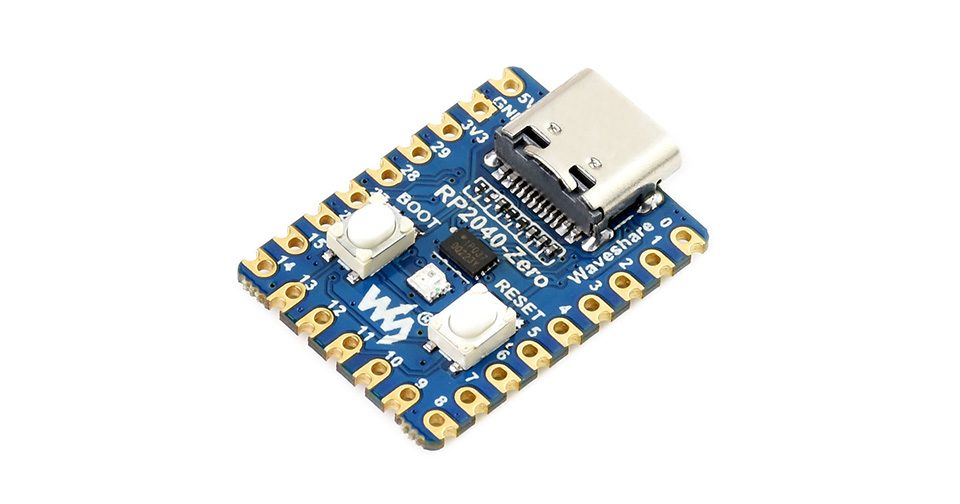
\includegraphics[width=0.7\linewidth]{Imagenes/Anexo_C/RP2040 Zero.png}
                \caption{RP2040 Zero}
                \label{fig:c1}
            \end{figure}
            
            Datos:\par
                \begin{itemize}[label=•]
                    \setlength{\itemindent}{2em}
                    
                    \item Chip microcontrolador RP2040 diseñado por Raspberry Pi en el Reino Unido\par
                    \item Procesador núcleo dual ARM Cortex M0+, con clock flexible que llega hasta los 133MHz\par
                    \item 264KB de SRAM, y 2MB de memoria Flash en la placa.
                    \item Conector USB-C, lo mantiene actualizado a los estándares actuales y más fácil de usar.\par
                    \item Los agujeros almenados permiten la soldadura directa a la placa.\par
                    \item USB 1.1 con soporte dispositivo/host.\par
                    \item Modos de suspención de bajo consumo y modo sleep.\par
                    \item Programación Drag-and-drop utilizando almacenaje en masa por USB.\par
                    \item 29 × pines GPIO multifunción (20× por vías externas, otros por puntos de soldadura).\par
                    \item 2 × SPI, 2 × I2C, 2 × UART, 4 × 12-bit ADC, 16 × canales de PWM controlables.\par
                    \item Clock y timer precisos en el chip.\par
                    \item Sensor de Temperatura.\par
                    \item Librerías     Accelerated floating-point en el chip.\par
                    \item 8 × Programmable I/O (PIO) state machines para soporte de periféricos personalizados.\par
                \end{itemize}
            
                Sitio Web: (\href{https://www.waveshare.com/wiki/RP2040-Zero}{https://www.waveshare.com/wiki/RP2040-Zero})\par
        
        \newpage
        
        \section{INA219}
        \label{ina219}
                \begin{figure}[!ht]
                    \centering
                    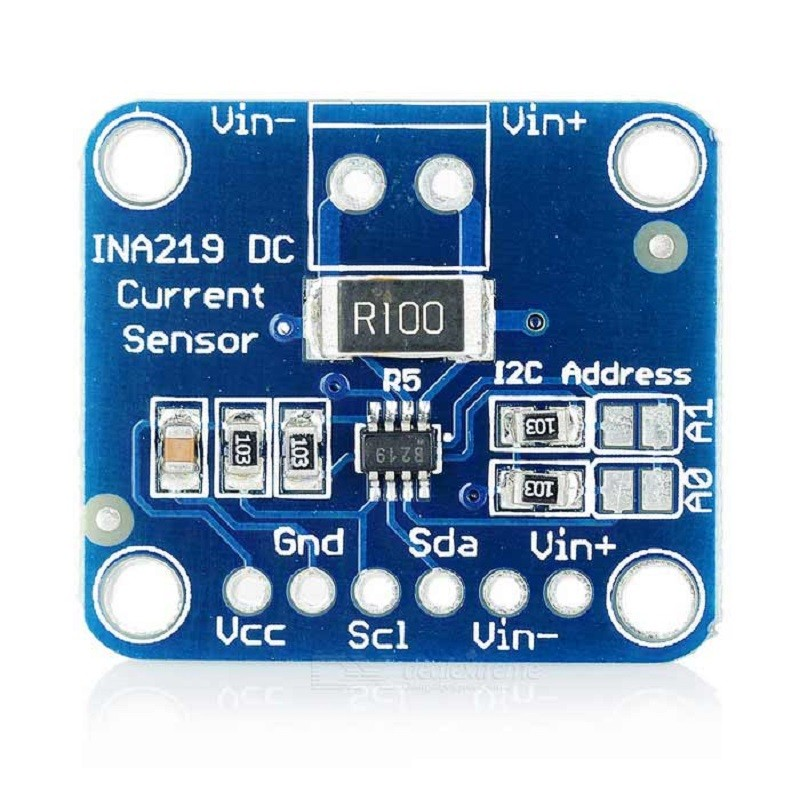
\includegraphics[width=0.7\linewidth]{Imagenes/Anexo_C/INA219.png}
                    \caption{Módulo INA219}
                    \label{fig:c2}
                \end{figure}
            
                Datos:\par
            
                \begin{itemize}[label=•]
                    \setlength{\itemindent}{2em}
                    
                    \item Entrada de potencia: 3,0V-5,5V\par
                    \item Voltaje objetivo hasta +26V\par
                    \item Resistencia de detección de corriente de 0,1 ohm 1\% 2W\par
                    \item Medición de corriente de hasta ±3,2A, con resolución de ±0,8mA\par
                    \item Detecta voltajes de bus de 0 a 26 V\par
                    \item Interfaz compatible con I2C- o SMBus-\par
                    \item Se pueden promediar hasta 128 muestras para lograr filtrado en entornos ruidosos.\par
                    \item Dimensiones de la Placa: 0.8 x 0.9 Pulgadas (l x w x h)\par
                \end{itemize}
            
                Datasheet: (\href{https://www.alldatasheet.com/datasheet-pdf/pdf/249609/TI/INA219.html}{https://www.alldatasheet.com/datasheet-pdf/pdf/249609/TI/INA219.html})\par

        \newpage
        
        \section{LPD3806-360BM}
        \label{encoder}
        
                \begin{figure}[!ht]
                \centering
                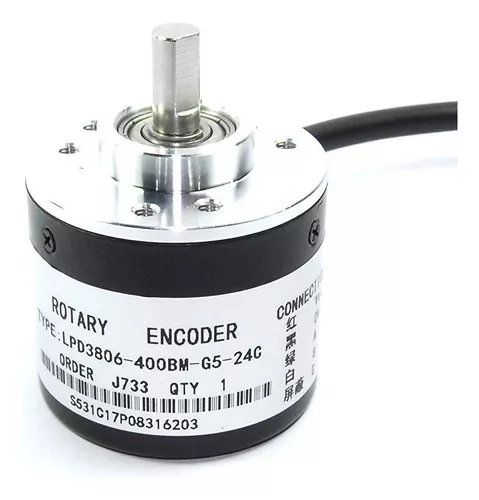
\includegraphics[width=0.5\linewidth]{Imagenes/Anexo_C/Encoder.png}
            \caption{LPD3806-360BM}
            \label{fig:c3}
        \end{figure}
        
            Datos:\par
            
            \begin{itemize}[label=•]
                \setlength{\itemindent}{2em}
                
                \item Pulsos: 600 p/r (600 pulsos/R monofasico, doble frecuencia de 4 a 2400 pulsos).\par
                \item Tension de Funcionamiento: 5V a 24V DC
                \item Eje: 6mm (Diametro) x 13mm (Largo)\par
                \item Dimensiones: 38mm x 35,5mm\par
                \item Salida de Pulso ortogonal rectangular con salida 2 fases AB\par
                \item Salida de colector abierto NPN\par
                \item Velocidad Mecanica Maxima: 5000rpm.\par
                \item Frecuencia de respuesta: 0-20kHz\par
            \end{itemize}
            
            Datasheet: (\href{https://www.alldatasheet.com/datasheet-pdf/pdf/1150705/ETC2/LPD3806-360BM.html}{https://www.alldatasheet.com/datasheet-pdf/pdf/1150705/ETC2/LPD3806-360BM.html}) (Está en Chino)\par

    \newpage
    
    \section{ESP8266 ESP-01S}
    \label{esp8266}
        \begin{figure}[!ht]
            \centering
            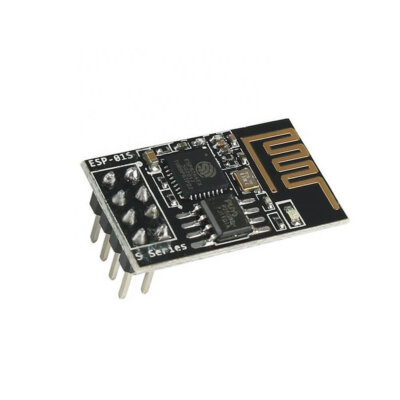
\includegraphics[width=0.5\linewidth]{Imagenes/Anexo_C/ESP8266.png}
            \caption{Módulo ESP8266 ESP-01S}
            \label{fig:c4}
        \end{figure}
        
        Datos:\par
        
        \begin{itemize}[label=•]
            \setlength{\itemindent}{2em}
            
            \item Voltaje de alimentación: 3.3 V. Este módulo no tolera 5 V.\par
            \item Comunicación tipo de interfaz: Serial, UART\par
            \item CPU de 32 bits\par
            \item Frecuencia de Reloj: 80MHz/160MHz\par
           \item Instruction RAM: 32KB\par
            \item Data RAM: 96KB\par
            \item Memoria Flash Externa: 4MB\par
            \item Soporte 3 modos: AP, STA, AP + STA\par
            \item Wi-Fi Direct (P2p), soft-AP\par
            \item Protocolos soportados: 802.11 b/g/n –  TCP/IP\par
            \item Soporte de red: 2,4 GHz\par
            \item Perfecto y simple en comandos AT\par
        \end{itemize}
            
        Datasheet: (\href{https://www.alldatasheet.com/datasheet-pdf/pdf/1424861/ETC/ESP8266.html}{https://www.alldatasheet.com/datasheet-pdf/pdf/1424861/ETC/ESP8266.html})\par